\documentclass[usenames,dvipsnames,smaller%,handout
]{beamer}
% \usepackage[T1]{fontenc} 
% \usepackage{lmodern} 
%\usepackage{etex}
%\newcommand{\num}{6{} }

% \usetheme[
%   outer/progressbar=foot,
%   outer/numbering=fraction,
%   block=fill,
%   inner/subsectionpage=progressbar
% ]{metropolis}
\usetheme{Madrid}
\useoutertheme[subsection=false]{miniframes} % Alternatively: miniframes, infolines, split
\useinnertheme{circles}
%\useoutertheme{Frankfurt}
\usecolortheme{beaver}
%\useoutertheme{crane}
%\useoutertheme{metropolis}
\usepackage[backend=biber,style=authoryear,maxcitenames=2,maxbibnames=99,safeinputenc,url=false,
eprint=false]{biblatex}
\addbibresource{bib/references.bib}
\AtEveryCitekey{\iffootnote{{\tiny}\tiny}{\tiny}}

\usepackage{pgfpages}
%\setbeameroption{hide notes} % Only slides
%\setbeameroption{show only notes} % Only notes
\setbeameroption{hide notes} % Only notes
%\setbeameroption{show notes on second screen=right} % Both
\usepackage{appendixnumberbeamer}
% \usepackage[sfdefault]{Fira Sans}

% \setsansfont[BoldFont={Fira Sans}]{Fira Sans Light}
% \setmonofont{Fira Mono}

%\usepackage{fira}
%\setsansfont{Fira}
%\setmonofont{Fira Mono}
% To give a presentation with the Skim reader (http://skim-app.sourceforge.net) on OSX so
% that you see the notes on your laptop and the slides on the projector, do the following:
% 
% 1. Generate just the presentation (hide notes) and save to slides.pdf
% 2. Generate onlt the notes (show only nodes) and save to notes.pdf
% 3. With Skim open both slides.pdf and notes.pdf
% 4. Click on slides.pdf to bring it to front.
% 5. In Skim, under "View -> Presentation Option -> Synhcronized Noted Document"
%    select notes.pdf.
% 6. Now as you move around in slides.pdf the notes.pdf file will follow you.
% 7. Arrange windows so that notes.pdf is in full screen mode on your laptop
%    and slides.pdf is in presentation mode on the projector.

% Give a slight yellow tint to the notes page
\setbeamertemplate{note page}{\pagecolor{yellow!5}\insertnote}\usepackage{palatino}

%\usetheme{metropolis}
%\usecolortheme{beaver}
\usepackage{tipa}
\definecolor{darkcandyapplered}{HTML}{A40000}
\definecolor{lightcandyapplered}{HTML}{e74c3c}

%\setbeamercolor{title}{fg=darkcandyapplered}

\definecolor{UBCblue}{rgb}{0.04706, 0.13725, 0.26667} % UBC Blue (primary)
\definecolor{UBCgrey}{rgb}{0.3686, 0.5255, 0.6235} % UBC Grey (secondary)

% \setbeamercolor{palette primary}{bg=darkcandyapplered,fg=white}
% \setbeamercolor{palette secondary}{bg=darkcandyapplered,fg=white}
% \setbeamercolor{palette tertiary}{bg=darkcandyapplered,fg=white}
% \setbeamercolor{palette quaternary}{bg=darkcandyapplered,fg=white}
% \setbeamercolor{structure}{fg=darkcandyapplered} % itemize, enumerate, etc
% \setbeamercolor{section in toc}{fg=darkcandyapplered} % TOC sections
% \setbeamercolor{frametitle}{fg=darkcandyapplered,bg=white} % TOC sections
% \setbeamercolor{title in head/foot}{bg=white,fg=white} % TOC sections
% \setbeamercolor{button}{fg=darkcandyapplered} % TOC sections

% % Override palette coloring with secondary
% \setbeamercolor{subsection in head/foot}{bg=lightcandyapplered,fg=white}

%\usecolortheme{crane}
% \makeatletter
% \setbeamertemplate{headline}{%
%   \begin{beamercolorbox}[colsep=1.5pt]{upper separation line head}
%   \end{beamercolorbox}
%   \begin{beamercolorbox}{section in head/foot}
%     \vskip1pt\insertsectionnavigationhorizontal{\paperwidth}{}{}\vskip1pt
%   \end{beamercolorbox}%
%   \ifbeamer@theme@subsection%
%     \begin{beamercolorbox}[colsep=1.5pt]{middle separation line head}
%     \end{beamercolorbox}
%     \begin{beamercolorbox}[ht=2.5ex,dp=1.125ex,%
%       leftskip=.3cm,rightskip=.3cm plus1fil]{subsection in head/foot}
%       \usebeamerfont{subsection in head/foot}\insertsubsectionhead
%     \end{beamercolorbox}%
%   \fi%
%   \begin{beamercolorbox}[colsep=1.5pt]{lower separation line head}
%   \end{beamercolorbox}
% }
% \makeatother

\setbeamertemplate{frametitle}{%
    \nointerlineskip%
    \begin{beamercolorbox}[wd=\paperwidth,ht=2.0ex,dp=0.6ex]{frametitle}
        \hspace*{1ex}\insertframetitle%
    \end{beamercolorbox}%
}


%\setbeamercolor{frametitle}{bg=darkcandyapplered!80!black!90!white}
%\setbeamertemplate{frametitle}{\bf\insertframetitle}

%\setbeamercolor{footnote mark}{fg=darkcandyapplered}
%\setbeamercolor{footnote}{fg=darkcandyapplered!70}
%\Raggedbottom
%\setbeamerfont{page number in head/foot}{size=\tiny}
%\usepackage[tracking]{microtype}


%\usepackage[sc,osf]{mathpazo}   % With old-style figures and real smallcaps.
%\linespread{1.025}              % Palatino leads a little more leading

% Euler for math and numbers
%\usepackage[euler-digits,small]{eulervm}
%\AtBeginDocument{\renewcommand{\hbar}{\hslash}}
\usepackage{graphicx,multirow,paralist,booktabs}


\mode<presentation> { \setbeamercovered{transparent} }

\setbeamertemplate{navigation symbols}{}
\makeatletter
\def\beamerorig@set@color{%
  \pdfliteral{\current@color}%
  \aftergroup\reset@color
}
\def\beamerorig@reset@color{\pdfliteral{\current@color}}
\makeatother


%=== GRAPHICS PATH ===========
\graphicspath{{./images/}}
% Marginpar width
%Marginpar width
%\setlength{\marginparsep}{.02in}


%% Captions
% \usepackage{caption}
% \captionsetup{
%   labelsep=quad,
%   justification=raggedright,
%   labelfont=sc
% }

\setbeamerfont{caption}{size=\footnotesize}
\setbeamercolor{caption name}{fg=darkcandyapplered}

%AMS-TeX packages

\usepackage{amssymb,amsmath,amsthm,mathtools} 
\usepackage{bm}
\usepackage{color}

%https://tex.stackexchange.com/a/31370/2269
\usepackage{mathtools,cancel}

\renewcommand{\CancelColor}{\color{red}} %change cancel color to red

\makeatletter
\let\my@cancelto\cancelto %copy over the original cancelto command
\newcommand<>{\cancelto}[2]{\alt#3{\my@cancelto{#1}{#2}}{\mathrlap{#2}\phantom{\my@cancelto{#1}{#2}}}}
% redefine the cancelto command, using \phantom to assure that the
% result doesn't wiggle up and down with and without the arrow
\makeatother


\usepackage{comment}
%\usepackage{hyperref,enumerate}
\usepackage{minitoc,array,enumerate}

\definecolor{slblue}{rgb}{0,.3,.62}
% \hypersetup{
%     colorlinks,%
%     citecolor=blue,%
%     filecolor=blue,%
%     linkcolor=blue,
%     urlcolor=slblue
% }

\usepackage{epstopdf}
\epstopdfDeclareGraphicsRule{.gif}{png}{.png}{convert gif:#1 png:\OutputFile}
\AppendGraphicsExtensions{.gif}

\usepackage{listings}

%%% TIKZ
\usepackage{forest}
\usepackage{tikz}
\usepackage{tikz-3dplot}
\usepackage{pgfplots}
\usepackage{pgfplotstable}
% \usepackage{pgfgantt}
\usepackage{neuralnetwork}
\pgfplotsset{compat=newest}

\usetikzlibrary{fit,arrows,shapes,positioning,chains,shapes.geometric}
\usetikzlibrary{decorations.markings}
\usetikzlibrary{shadows,automata}
\usetikzlibrary{patterns}
\usetikzlibrary{trees,mindmap,backgrounds}
%\usetikzlibrary{circuits.ee.IEC}
\usetikzlibrary{decorations.text}
% For Sagnac Picture
\usetikzlibrary{%
    decorations.pathreplacing,%
    decorations.pathmorphing%
}
\tikzset{no shadows/.style={general shadow/.style=}}
%
%\usepackage{paralist}

\tikzset{
  font=\Large\sffamily\bfseries,
  red arrow/.style={
    midway,red,sloped,fill, minimum height=3cm, single arrow, single arrow head extend=.5cm, single arrow head indent=.25cm,xscale=0.3,yscale=0.15,
    allow upside down
  },
  black arrow/.style 2 args={-stealth, shorten >=#1, shorten <=#2},
  black arrow/.default={1mm}{1mm},
  tree box/.style={draw, rounded corners, inner sep=1em},
  node box/.style={white, draw=black, text=black, rectangle, rounded corners},
}

%%% FORMAT PYTHON CODE
%\usepackage{listings}
% Default fixed font does not support bold face
\DeclareFixedFont{\ttb}{T1}{txtt}{bx}{n}{8} % for bold
\DeclareFixedFont{\ttm}{T1}{txtt}{m}{n}{8}  % for normal

% Custom colors
\definecolor{deepblue}{rgb}{0,0,0.5}
\definecolor{deepred}{rgb}{0.6,0,0}
\definecolor{deepgreen}{rgb}{0,0.5,0}

\usepackage{animate}

% Python style for highlighting
% \newcommand\pythonstyle{\lstset{
% language=Python,
% basicstyle=\footnotesize\ttm,
% otherkeywords={self},             % Add keywords here
% keywordstyle=\footnotesize\ttb\color{deepblue},
% emph={MyClass,__init__},          % Custom highlighting
% emphstyle=\footnotesize\ttb\color{deepred},    % Custom highlighting style
% stringstyle=\color{deepgreen},
% frame=tb,                         % Any extra options here
    % showstringspaces=false            % 
% }}

% % Python environment
% \lstnewenvironment{python}[1][]
% {
% \pythonstyle
% \lstset{#1}
% }
% {}

% % Python for external files
% \newcommand\pythonexternal[2][]{{
% \pythonstyle
% \lstinputlisting[#1]{#2}}}

% Python for inline
% 
% \newcommand\pythoninline[1]{{\pythonstyle\lstinline!#1!}}

%\usepackage{algorithm2e}

\newcommand{\eps}{\epsilon}
\newcommand{\bX}{\mb X}
\newcommand{\by}{\mb y}
\newcommand{\bbe}{\bm\beta}
\newcommand{\beps}{\bm\epsilon}
\newcommand{\bY}{\mb Y}

\newcommand{\osn}{\oldstylenums}
\newcommand{\dg}{^{\circ}}
\newcommand{\lt}{\left}
\newcommand{\rt}{\right}
\newcommand{\pt}{\phantom}
\newcommand{\tf}{\therefore}
\newcommand{\?}{\stackrel{?}{=}}
\newcommand{\fr}{\frac}
\newcommand{\dfr}{\dfrac}
\newcommand{\ul}{\underline}
\newcommand{\tn}{\tabularnewline}
\newcommand{\nl}{\newline}
\newcommand\relph[1]{\mathrel{\phantom{#1}}}
\newcommand{\cm}{\checkmark}
\newcommand{\ol}{\overline}
\newcommand{\rd}{\color{red}}
\newcommand{\bl}{\color{blue}}
\newcommand{\pl}{\color{purple}}
\newcommand{\og}{\color{orange!90!black}}
\newcommand{\gr}{\color{green!40!black}}
\newcommand{\lbl}{\color{CornflowerBlue}}
\newcommand{\dca}{\color{darkcandyapplered}}
\newcommand{\nin}{\noindent}
\newcommand*\circled[1]{\tikz[baseline=(char.base)]{
            \node[shape=circle,draw,thick,inner sep=1pt] (char) {\small #1};}}

\newcommand{\bc}{\begin{compactenum}[\quad--]}
\newcommand{\ec}{\end{compactenum}}

\newcommand{\p}{\partial}
\newcommand{\pd}[2]{\frac{\partial{#1}}{\partial{#2}}}
\newcommand{\dpd}[2]{\dfrac{\partial{#1}}{\partial{#2}}}
\newcommand{\pdd}[2]{\frac{\partial^2{#1}}{\partial{#2}^2}}
\newcommand{\pde}[3]{\frac{\partial^2{#1}}{\partial{#2}\partial{#3}}}
\newcommand{\nmfr}[3]{\Phi\left(\frac{{#1} - {#2}}{#3}\right)}
\newcommand{\Err}{\text{Err}}
\newcommand{\err}{\text{err}}

\DeclarePairedDelimiter\ceil{\lceil}{\rceil}
\DeclarePairedDelimiter\floor{\lfloor}{\rfloor}

%%%% GREEK LETTER SHORTCUTS %%%%%
\newcommand{\la}{\lambda}
\renewcommand{\th}{\theta}
\newcommand{\al}{\alpha}
\newcommand{\G}{\Gamma}
\newcommand{\si}{\sigma}
\newcommand{\Si}{\Sigma}

\pgfmathdeclarefunction{poiss}{1}{%
  \pgfmathparse{(#1^x)*exp(-#1)/(x!)}%
  }

\pgfmathdeclarefunction{gauss}{2}{%
  \pgfmathparse{1/(#2*sqrt(2*pi))*exp(-((x-#1)^2)/(2*#2^2))}%
}


% \usepackage{pst-plot}

% \usepackage{pstricks-add}
% \usepackage{auto-pst-pdf}   

% \psset{unit = 3}

% \def\target(#1,#2){%
%  {\psset{fillstyle = solid}
%   \rput(#1,#2){%
%     \pscircle[fillcolor = white](0.7,0.7){0.7}
%     \pscircle[fillcolor = blue!60](0.7,0.7){0.5}
%     \pscircle[fillcolor = white](0.7,0.7){0.3}
%     \pscircle[fillcolor = red!80](0.7,0.7){0.1}}}}
% \def\dots[#1](#2,#3){%
%     \psRandom[
%       dotsize = 2pt,
%       randomPoints = 25
%     ](!#2 #1 0.04 sub sub #3 #1 0.04 sub sub)%
%      (!#2 #1 0.04 sub add #3 #1 0.04 sub add)%
%      {\pscircle[linestyle = none](#2,#3){#1}}}





%%%%%%%%%%%%%%%%%%%%%%%%%%%%%%%%%%%%%%%%%%%%%%%%%%%
%%%%%%%%%%%%%%%%%%%%%%%%%%%%%%%%%%%%%%%%%%%%%%%%%%%

\title[AI Trees: Intro]{ {\normalsize Artificial Intelligence for Tree Failure Identification and Risk Quantification}
  \\ Introductory Meeting}
\date[\today]{\footnotesize \today}
\author{{\bf NARS Lab}}
\institute[UMass Amherst]{
%\titlegraphic{\hfill
  \begin{tikzpicture}[baseline=(current bounding box.center)]
    \node[anchor=base] at (-7,0) (its) {\includegraphics[scale=.3]{UMassEngineering_vert}} ;
  \end{tikzpicture}
  % \hfill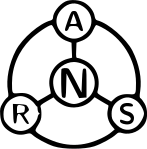
\includegraphics[height=1.5cm]{logo}
}

%https://tex.stackexchange.com/questions/55806/mindmap-tikzpicture-in-beamer-reveal-step-by-step
  \tikzset{
    invisible/.style={opacity=0},
    visible on/.style={alt={#1{}{invisible}}},
    alt/.code args={<#1>#2#3}{%
      \alt<#1>{\pgfkeysalso{#2}}{\pgfkeysalso{#3}} % \pgfkeysalso doesn't change the path
    },
  }


% https://tex.stackexchange.com/questions/446468/labels-with-arrows-for-an-equation
% https://tex.stackexchange.com/a/402466/121799
\newcommand{\tikzmark}[3][]{
\ifmmode
\tikz[remember picture,baseline=(#2.base)] \node [inner sep=0pt,#1](#2) {$#3$};
\else
\tikz[remember picture,baseline=(#2.base)] \node [inner sep=0pt,#1](#2) {#3};
\fi
}

\lstset{language=matlab,
                basicstyle=\scriptsize\ttfamily,
                keywordstyle=\color{blue}\ttfamily,
                stringstyle=\color{blue}\ttfamily,
                commentstyle=\color{gray}\ttfamily,
                morecomment=[l][\color{gray}]{\#}
              }

              
\begin{document}

\maketitle

% \begin{frame}
%   \frametitle{Second half of the semester}
%   \pause
%   Modules to be covered in the next 4 weeks: \\ \pause
%   \begin{enumerate}[<+->]\setcounter{enumi}{6}
%   \item Tree-based methods
%   \item Support Vector Machines (SVM)
%   \item Neural Networks
%   \item Unsupervised Learning
%     \begin{itemize}[<+->]
%     \item Principal components analysis (PCA)
%     \item Clustering analysis
%     \end{itemize}
%   \end{enumerate}

%   \pause

%   \textbf{Project}\pause
%   \begin{itemize}
%   \item Check Moodle for instructions; proposals due April 10
%   \end{itemize}
%   \pause

%   \medskip
  
%   \textbf{Final Exam}\pause
%   \begin{itemize}
%   \item Cumulative 24-hr open-book take-home exam.
%   \end{itemize}
% \end{frame}

\begin{frame}
  \frametitle{Outline}\small
  \tableofcontents
\end{frame}

 

\section{Convolutional NNs}
\begin{frame}
  \frametitle{The convolutional neural network (CNN)}
  \pause

  \begin{itemize}
  \item Motivated by the image recognition process of the brain's visual cortex.

  \item Groundbreaking study on cats revealed the importance of \textit{local receptive fields} for activating neurons
    in the visual cortex. (Hubel \& Wiesel, 1958; 1959)

  \item Earliest neural network for image recognitron introduced: \textit{neocognitron} (Fukushima, 1980)

  \item Milestone: introduction of \textit{LeNet-5} architecture for handwritten digit recognition (Yann LeCun et al., 1998)
  \end{itemize}
  
\end{frame}

\begin{frame}
  \frametitle{Building blocks of a CNN}

  \begin{itemize}
  \item \textbf{Input layer:} the image to be classified 
  \item \textbf{Convolutional layer:} represents the action of a filter transmitting signals (features) from various
    portions (receptive fields) of the preceding layer. The size of the receptive field is specified by the
    \textit{convolutional kernel}. Each layer can have multiple feature maps representing different filters.
  \item \textbf{Pooling layer:} subsamples signals from preceding layer to reduce dimensionality and extract dominant
    features (subsample space determined by kernel size)
  \item \textbf{Dense layer:} neuron outputs are flattened and fully connected %(usually with decreasing number of neurons)
  \item \textbf{Output layer:} neurons equal to number of classes; with softmax activation
  \end{itemize}

  \begin{center}
    \includegraphics[width=.6\textwidth]{cnn-ex1}
  \end{center}

  {\tiny Source: \url{https://neurdiness.wordpress.com/2018/05/17/deep-convolutional-neural-networks-as-models-of-the-visual-system-qa/}}

  
\end{frame}

\begin{frame}
  \frametitle{Training hyperparameters in a CNN}
  Several decisions must be made in selecting hyperparameters for training a CNN.

  \begin{itemize}
  \item Number of convolutional layers and feature maps in each layer
  \item Convolutional kernel size
  \item Stride length (spacing of filters)
  \item Choice of pooling function (max, average, etc)
  \item Number of dense layers
  \item Activation function in each layer (ReLU, tanh, etc)
  \end{itemize}

  Various high-performing architectures have been developed in recent years that can be adapted for other problems.

  Training the network involves finding the weights for the various layers (using mini-batch gradient descent or other variants)
\end{frame}


% \section{AI for Tree Risk}
% \begin{frame}
%   \frametitle{Automating tree risk prediction using AI}

%   \begin{itemize}
%   \item \textbf{Objective:}  Automate tree risk classification using a convolutional neural network?
%   \item \textbf{Question 1:} Can we elicit the visual features from a trained network that indicate various levels of risk?
%   \item \textbf{Question 2:} Can we map estimated CNN weights to structural relationships governing tree stability?
%   \item \textbf{Question 3:} How well can a trained CNN be transferred to another set of images and perform similarly well for risk prediction?
%   \item \textbf{Question 4:} How can this process be adapted for Google Maps images (or drone photography)?
%   \end{itemize}
% \end{frame}

\section{Methods and Results}
\begin{frame}
  \frametitle{Data preprocessing}
  \pause

  \begin{itemize}[<+->]
  \item Labeled 458 images serially and by class:\pause
    \begin{itemize}
    \item Probable images saved: 56
    \item Possible images saved: 80      
    \item Improbable images saved: 322
    \end{itemize}
  \item Cropped images to $3024 \times 3024$%\footnote{More rigorous checking required to ensure that relevant features were not cropped out.}
  \item Downsampled to $108 \times 108$ (using standard cubic interpolation algorithm)\pause
    \begin{center}
      \includegraphics[width=.5\textwidth]{image0.png}
    \end{center}
  \item Randomly split images into training and validation sets (80:20 ratio)\pause
    \begin{itemize}
    \item Size of validation sample: 76 images
    \end{itemize}
  \end{itemize}
\end{frame}
\begin{frame}
  \frametitle{CNN Model 1 }
  \begin{minipage}{.45\linewidth}
    \begin{itemize}[<+->]
      \item Binary image classifier
  \item Simple architecture:
    \begin{itemize}
    \item 5 convolutional layers
    \item 2 hidden dense layers
    \item 1 output layer
  \end{itemize}
  \item Input layer: $108\times108\times1$ tensor
  \item Output layer: $2\times 1$ vector of probabilities (of the input belonging to either of the classes)
  \end{itemize}
\end{minipage}
\pause
\begin{minipage}{.45\linewidth}
  \hspace{6ex}
  \includegraphics[width=.45\textwidth]{cnn-model1}
\end{minipage}
\end{frame}

\begin{frame}
  \frametitle{Training hyperparameters and decisions}
  \begin{itemize}[<+->]
  \item \textbf{Optimizer:} algorithm used for finding optimal CNN weights (usually a variant of stochastic gradient descent)
  \item \textbf{Batch size:} number of images used in each iteration to compute the gradients and update CNN weights
  \item \textbf{Epochs:} number of sweeps through all the training observations for CNN learning
  \item \textbf{Loss function:} quantifies the error in a prediction compared to the observed label
  \end{itemize}
\end{frame}

\begin{frame}
  \frametitle{Results}
  \pause

  Current results are based on Model 1 using monochromatic images, 4 epochs (algorithm converges fast) and 32 samples per batch. \pause

  \begin{itemize}[<+->]
  \item Optimizer used: Adam (variant of SGD)
  \item All performance metrics are based on validation set:\pause
    \begin{itemize}
    \item Precision: $\fr{TP}{TP + FP}$
    \item Recall: $\fr{TP}{TP + FN}$
    \end{itemize}
  \end{itemize}
  \pause
  
  \begin{tabular}{l l l l l}\toprule
    \bf Class Labels & \bf Image Size &\bf Prec. &\bf Recall &\bf Acc. \\ \midrule
    \{(Probable + Possible), Improbable\} & $108\times108$ &   &  & 65.2 \\\midrule \pause
    \{Probable, Possible, Improbable\} & $108\times108$ &   &  & 72.8 \\\midrule \pause
    \{Probable, Improbable\} & $108\times108$ & 87.9 & 100 & 86.8 \\\midrule\pause
    \{Probable, Improbable\} & $224\times224$ & 87.9 & 100 & 86.8 \\\bottomrule
  \end{tabular}
\end{frame}

\begin{frame}
  \frametitle{Results summary}
  \begin{itemize}[<+->]
  \item We obtained the best performance from a binary classification of Probable and Improbable images
  \item Increasing pixel size (108 to 224) did not improve results
  \end{itemize}
\end{frame}

\begin{frame}
  \frametitle{Next steps}
  \begin{itemize}[<+->]
  \item Implement a high-performance CNN architecture (usually deeper is better). Candidates: \pause
    \begin{itemize}
    \item ResNet50 (50 layers)
    \item GoogLeNet (22 layers)
    \end{itemize}

  \item \str Investigate effects of using 3 channels (full-color images) in training

  \item Explore data augmentation procedures
    
  \item Longer term: perform inferential interpretation of relevant features in trained CNN and map to physical relationships

  \item Compare trained assessments (professional opinion)
  \end{itemize}
\end{frame}

\appendix
\section{Backpropagation}

\begin{frame}
  \frametitle{Equation summary: outer layer}
  \pause
  At the outer layer $L$ (without indexing by neuron):\pause
  \begin{align}
    z^{(L)} &= w^{(L)} \times a^{(L-1)} + b^{(L)} \\\pause
    a^{(L)} &= \sigma(z^{(L)}) \\\pause
    C &= (a^{(L)}  - y)^2
  \end{align}
  \pause
  
  The gradient of the cost function with respect to $w^{(L)}$ is:\pause
  \begin{equation}
    \frac{\partial C}{\partial w^{(L)}}
    =\pause
    \frac{\partial C}{\partial a^{(L)}}
    \frac{\partial a^{(L)}}{\partial z^{(L)}}
    \frac{\partial z^{(L)}}{\partial w^{(L)}}
    =\pause
    2 \left(a^{(L)} - y \right) \sigma' \left(z^{(L)}\right) a^{(L-1)}
  \end{equation}
  \pause
  Thus, we see that this gradient depends on the activation from the previous layer $a^{(L-1)}$. \pause Also wrt to the bias:
  \begin{equation}
    \pd{C}{b^{(L)}} = \pause \pd{C}{a^{(L)}}\pd{a^{(L)}}{z^{(L)}}\pd{z^{(L)}}{b^{(L)}} =\pause 2\lt(a^{(L)} - y\rt)\sigma'(z^{(L)})(1)
  \end{equation}
\end{frame}

\begin{frame}
  \frametitle{Updating weights}
  \pause
  We can then update the weights for the last layer for the next iteration $r+1$:\pause
  \begin{align}
    w^{(L), r+1}  &=  w^{(L),r} - \eta \pd{C}{w^{(L)}}  \\\pause
    b^{(L), r+1}  &=  b^{(L),r} - \eta \pd{C}{b^{(L)}}  
  \end{align}
  \pause
  To update the weights for layer $L-1$, we need to find the gradients $\pd{C}{w^{(L-1)}}$ and $\pd{C}{b^{(L-1)}}$.

  \pause

  \medskip
  
  Using the chain rule again, we write:\pause
  \begin{align}
    \pd{C}{w^{(L-1)}} &= {\rd \pd{C}{a^{(L-1)}}}\pd{a^{(L-1)}}{z^{(L-1)}}\pd{z^{(L-1)}}{w^{(L-1)}} \\\pause
    \pd{C}{b^{(L-1)}} &= {\rd \pd{C}{a^{(L-1)}}}\pd{a^{(L-1)}}{z^{(L-1)}}\pd{z^{(L-1)}}{b^{(L-1)}} 
  \end{align}
\end{frame}

\begin{frame}
  \frametitle{Backward pass}
  \pause
  But we recall that $C$ is not \textit{explicitly} dependent on $a^{(L-1)}$ as $C = (a^{(L)} - y)^2$.
  \pause

  However, it is \textit{implicitly} dependent, since\pause
  \begin{equation}
    C \propto a^{(L)},
  \end{equation}
  \pause
  \begin{equation}
    a^{(L)} \propto z^{(L)} 
  \end{equation}
  \pause
  and\pause
  \begin{equation}
    z^{(L)} \propto a^{(L-1)}
  \end{equation}
  \pause
  
  So, we use the chain rule to expand $\pd{C}{a^{(L-1)}}$ as follows:\pause
  \begin{equation}\rd
    \pd{C}{a^{(L-1)}} = \pause \pd{C}{a^{(L)}}\pd{a^{(L)}}{z^{(L)}}\pd{z^{(L)}}{a^{(L-1)}}
  \end{equation}
\end{frame}

\begin{frame}
  \frametitle{Backward pass (cont.)}
  \pause
  We can then expand the cost function gradient wrt to weights for layer $L-1$ as:\pause
  \begin{align}
    \pd{C}{w^{(L-1)}} &= {\rd \pd{C}{a^{(L-1)}}}\pd{a^{(L-1)}}{z^{(L-1)}}\pd{z^{(L-1)}}{w^{(L-1)}} \pause
                        = {\rd \pd{C}{a^{(L)}}\pd{a^{(L)}}{z^{(L)}}\pd{z^{(L)}}{a^{(L-1)}}} \pd{a^{(L-1)}}{z^{(L-1)}}\pd{z^{(L-1)}}{w^{(L-1)}} \\[2mm]\pause
        \pd{C}{b^{(L-1)}} &= {\rd \pd{C}{a^{(L-1)}}}\pd{a^{(L-1)}}{z^{(L-1)}}\pd{z^{(L-1)}}{b^{(L-1)}} 
                            = {\rd \pd{C}{a^{(L)}}\pd{a^{(L)}}{z^{(L)}}\pd{z^{(L)}}{a^{(L-1)}}} \pd{a^{(L-1)}}{z^{(L-1)}}\pd{z^{(L-1)}}{b^{(L-1)}} 
  \end{align}

  \pause

  Once these gradients are computed, we update the weights for the $r+1$th iteration using: \pause
   \begin{align}
    w^{(L-1), r+1}  &= \pause  w^{(L-1),r} - \pause \eta \pd{C}{w^{(L-1)}}  \\\pause
    b^{(L-1), r+1}  &=  \pause b^{(L-1),r} - \pause \eta \pd{C}{b^{(L-1)}}  
  \end{align}
\end{frame}

\begin{frame}
  \frametitle{Summary: forward pass}
  \begin{enumerate}[<+->]
  \item Initialize weights and biases: $w^{(l),0}$, $b^{(l),0}$
  \item Perform forward pass to compute activations:
    \begin{align}
      z^{(l),0} &= w^{(l),0} \times a^{(l-1),0} + b^{(l),0} \\\pause
    a^{(l)} &= \sigma(z^{(l),0}) 
    \end{align}
    \pause
    At output layer:
    \begin{align}      
      z^{(L),0} &= w^{(L),0} \times a^{(L-1),0} + b^{(L),0} \\\pause
      a^{(L),0} &= \sigma(z^{(L),0}) \\
      C &= (a^{(L),0}  - y)^2
    \end{align}
  \end{enumerate}
\end{frame}

\begin{frame}
  \frametitle{Summary: backward pass---outer layer }
  \begin{enumerate}[<+->]\setcounter{enumi}{2}
  \item Backward pass, outer layer $(L)$:\pause
    \begin{enumerate}[<+->]
    \item Compute gradients: \pause
      \begin{align}
      \pd{C}{w^{(L)}} &= \pause \pd{C}{a^{(L)}}\pd{a^{(L)}}{z^{(L)}}\pd{z^{(L)}}{w^{(L)}}\\\pause
      \pd{C}{b^{(L)}} &= \pause \pd{C}{a^{(L)}}\pd{a^{(L)}}{z^{(L)}}\pd{z^{(L)}}{b^{(L)}}\pause
      \end{align}
    \item Update weights: \pause
      \begin{align}
        w^{(L), 1}  &=  w^{(L),0} - \eta \pd{C^0}{w^{(L)}}  \\\pause
      b^{(L), 1}  &=  b^{(L),0} - \eta \pd{C^0}{b^{(L)}}  
      \end{align}
  \end{enumerate}
  \end{enumerate}
\end{frame}

\begin{frame}
  \frametitle{Summary: backward pass---last hidden layer}
  \begin{enumerate}[<+->]\setcounter{enumi}{2}
  \item Backward pass, layer $(L-1)$:\pause
    \begin{enumerate}[<+->]\setcounter{enumii}{2}
    \item Compute gradients: \pause
    \begin{align}
      \pd{C}{w^{(L-1)}} &=  \pd{C}{a^{(L)}}\pd{a^{(L)}}{z^{(L)}}\pd{z^{(L)}}{a^{(L-1)}}  \pd{a^{(L-1)}}{z^{(L-1)}}\pd{z^{(L-1)}}{w^{(L-1)}}\\\pause
      \pd{C}{b^{(L-1)}} &=   \pd{C}{a^{(L)}}\pd{a^{(L)}}{z^{(L)}}\pd{z^{(L)}}{a^{(L-1)}} \pd{a^{(L-1)}}{z^{(L-1)}}\pd{z^{(L-1)}}{b^{(L-1)}}
    \end{align}
    \pause
  \item Update weights: \pause
    \begin{align}
      w^{(L-1), 1}  &= \pause  w^{(L-1),0} - \pause \eta \pd{C}{w^{(L-1)}}  \\\pause
      b^{(L-1), 1}  &=  \pause b^{(L-1),0} - \pause \eta \pd{C}{b^{(L-1)}}  
    \end{align}
  \end{enumerate}
  \end{enumerate}
\end{frame}

\begin{frame}
  \frametitle{Summary: backward pass---second-to-last hidden layer}
  \begin{enumerate}[<+->]\setcounter{enumi}{2}
  \item Backward pass, layer $(L-2)$:\pause
    \begin{enumerate}[<+->] \setcounter{enumii}{4}
    \item Compute gradients: \pause
    \begin{align}
      \pd{C}{w^{(L-2)}} &=  \pd{C}{a^{(L)}}\pd{a^{(L)}}{z^{(L)}}\pd{z^{(L)}}{a^{(L-1)}} \pause
                        \pd{a^{(L-1)}}{z^{(L-1)}}\pd{z^{(L-1)}}{a^{(L-2)}} \pause
                        \pd{a^{(L-2)}}{z^{(L-2)}}\pd{z^{(L-2)}}{w^{(L-2)}}\\\pause
      \pd{C}{b^{(L-2)}} &=   \pd{C}{a^{(L)}}\pd{a^{(L)}}{z^{(L)}}\pd{z^{(L)}}{a^{(L-1)}} \pause
                        \pd{a^{(L-1)}}{z^{(L-1)}}\pd{z^{(L-1)}}{a^{(L-2)}} \pause
                        \pd{a^{(L-2)}}{z^{(L-2)}}\pd{z^{(L-2)}}{b^{(L-2)}}\\\pause
    \end{align}
    \pause
  \item Update weights: \pause
    \begin{align}
      w^{(L-2), 1}  &= \pause  w^{(L-2),0} - \pause \eta \pd{C}{w^{(L-2)}}  \\\pause
      b^{(L-2), 1}  &=  \pause b^{(L-2),0} - \pause \eta \pd{C}{b^{(L-2)}}  
    \end{align}
  \end{enumerate}
  \end{enumerate}
\end{frame}


\begin{frame}
  \frametitle{Summary: backward pass---first hidden layer}
  \begin{enumerate}[<+->]\setcounter{enumi}{2}
  \item Backward pass, layer $(1)$:\pause
        \begin{enumerate}[<+->] \setcounter{enumii}{4}
    \item Compute gradients: \pause
    \begin{align}
      \pd{C}{w^{(1)}} &=  \pd{C}{a^{(L)}}\pd{a^{(L)}}{z^{(L)}}\pd{z^{(L)}}{a^{(L-1)}}\pd{a^{(L-1)}}{z^{(L-1)}} \pause
                          \pause\cdots  
                          \pd{z^{(2)}}{a^{(1)}}                          
                        \pd{a^{(1)}}{z^{(1)}}\pd{z^{(1)}}{w^{(1)}}\\\pause
      \pd{C}{b^{(1)}} &=  \pd{C}{a^{(L)}}\pd{a^{(L)}}{z^{(L)}}\pd{z^{(L)}}{a^{(L-1)}}\pd{a^{(L-1)}}{z^{(L-1)}} \pause
                          \pause\cdots  
                          \pd{z^{(2)}}{a^{(1)}}                          
                        \pd{a^{(1)}}{z^{(1)}}\pd{z^{(1)}}{b^{(1)}}\\\pause
    \end{align}
    \pause
  \item Update weights: \pause
    \begin{align}
      w^{(1), 1}  &= \pause  w^{(1),0} - \pause \eta \pd{C}{w^{(1)}}  \\\pause
      b^{(1), 1}  &=  \pause b^{(1),0} - \pause \eta \pd{C}{b^{(1)}}  
    \end{align}
  \end{enumerate}
  \end{enumerate}
\end{frame}
% \section{Summary}
% \begin{frame}[fragile]
%   \frametitle{Summary}
%   \pause
%   Today, we considered an introduction to neural networks. We will finalize this on Friday with real examples.
%   \begin{itemize}[<+->]
%   \item For now, you may play around with \href{http://playground.tensorflow.org}{\bl \bf this}
%     \item Reading: ESL 11.3 -- 11.6 (complete before next lecture); you will notice differences in notation used.
%   \end{itemize}
% \end{frame}

% \begin{frame}
%   \frametitle{Reading}\pause
%   Today's lecture:\pause
  
% \begin{itemize}[<+->]
% \item Support vector machines: ISLR 9.3, 9.4; ESL 12.3.1
% \item 
%   % \item Boosting: ESL 10 (Very dense chapter. You may want to focus on 10.1--10.3, 10.7, 10.10, 10.13, 10.14.)
% \end{itemize}
% \pause
% \bigskip
  

% \end{frame}
 
%http://www.di.fc.ul.pt/~jpn/r/rbf/rbf.html
\end{document}

%%% Local Variables:
%%% mode: latex
%%% TeX-master: t
%%% End:
